\documentclass[../main.tex]{subfiles}

\begin{document}

\section{Neutrinos}%
\label{sec:neutrinos}

Als bijnaam hebben de neutrinos de naam ``ghost'' particles. De reden hiervoor is dat ze alleen zwak interageren wat hen een kleine werkzame doorsnede geeft en dus moeilijk te detecteren zijn. Bij deze deeltjes hebben we een hoop vragen die nog niet opgelost zijn.
\begin{itemize}
    \item Zijn dit Dirac of Majorana fermionen?
    \item Wat is hun massa?
    \item Wat zijn hun oscillatie eigenschappen?
    \item Is er $CP$ schending in de lepton sector?
    \item Zijn er rechts handige neutrinos?
    \item Zijn er meer dan 3 types neutrinos?
\end{itemize}
Vandaag de dag hebben we enkel een antwoord op de vraag wat hun oscillatie eigenschappen zijn. Dit alles zullen we bespreken in dit hoofdstuk.

\subsection{Neutrino bronnen}%
\label{sub:neutrino_bronnen}

Door het moeilijk te detecteren zijn is het belangrijk dat we er veel aanmaken. De belangrijkste bronnen zijn:
\begin{itemize}
    \item Zonne neutrinos: Ontstaan uit nucleaire reacties in de zon en dus met een energie in de MeV's. Om te zien hoe de zon neutrinos maakt moeten we kijken naar hoe deze brandt. De zon zal protonen fuseren tot $^4He$ kernen ($pp$-cyclus).
        \begin{equation}
            \begin{aligned}
                \label{eq:zon_fusie}
                p+p & \rightarrow D+e^{+}+\nu_{e} \\
                D+p & \rightarrow{ }^{3} \mathrm{He}+\gamma \\
                { }^{3} \mathrm{He}+{ }^{3} \mathrm{He} & \rightarrow{ }^{4} \mathrm{H}{ }^{2}+p+p
            \end{aligned}
        \end{equation}
        We moeten hier uiteindelijk 4 protonen omzetten in 2 protonen en 2 neutronen. Dit omzetten kan enkel gebeuren via de zwakke wisselwerking. We mogen blij zijn dat de zon zal branden aan de hand van de zwakke wisselwerking omdat deze anders heel snel opgebrand zou zijn. Naast deze $pp$-cyclus hebben we ook nog de Boron-cycle
        \begin{equation}
            \begin{aligned}
                \label{eq:boron_cyclus}
                { }^{4} \mathrm{He}+{ }^{3} \mathrm{He} & \rightarrow{ }^{7} \mathrm{Be}+\gamma \\
                { }^{7} \mathrm{Be}+p & \rightarrow{ }^{8} \mathrm{~B}+\gamma \\
                { }^{8} \mathrm{~B} & \rightarrow{ }^{8} \mathrm{Be}^{*}+e^{+}+\nu_{e} \\
                { }^{8} \mathrm{Be}^{*} & \rightarrow{ }^{4} \mathrm{He}+{ }^{4} \mathrm{He}
            \end{aligned}
        \end{equation}
        waar terug een zwakke wisselwerking component zit, de Be-capture
        \begin{equation}
            \begin{aligned}
                \label{eq:be_capture}
                { }^{7} \mathrm{Be}+e^{-} \rightarrow^{7} \mathrm{Li}+\nu_{e}
            \end{aligned}
        \end{equation}
        wat een zwakke wisselwerking is en de $pep$ reactie
        \begin{equation}
            \begin{aligned}
                \label{eq:pep}
                p+e^{-}+p \rightarrow D+\nu_{e}
            \end{aligned}
        \end{equation}
        De 2 laatste processen zullen een non energetisch neutrino aanmaken. Zo ziet het neutrino spectrum er als volgt uit.

        \begin{figure}[h]
            \centering
            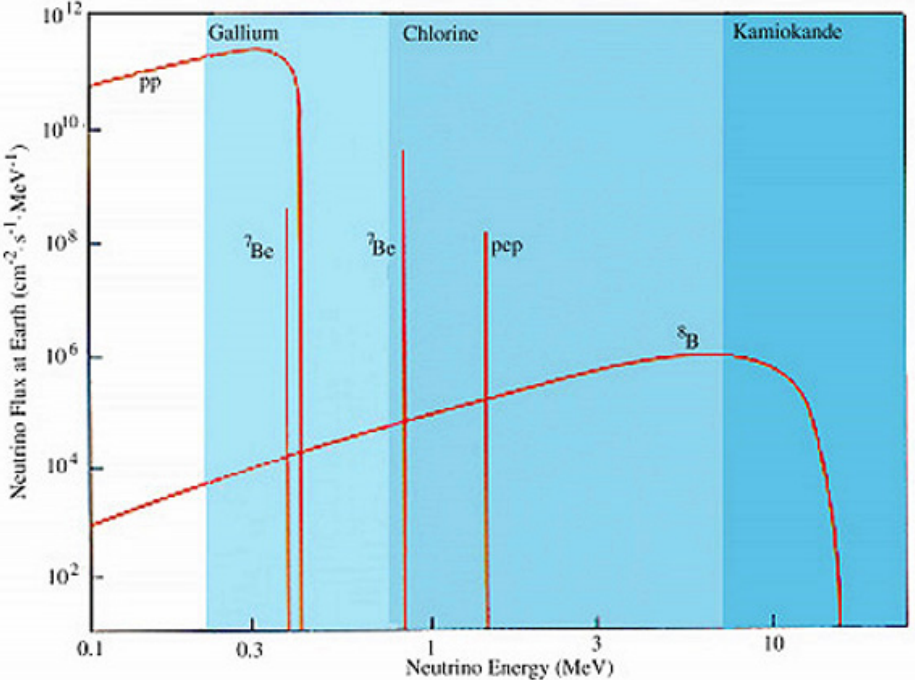
\includegraphics[width=0.5\linewidth]{neutrinos/zon_neutrino_spectrum.png}
            \caption{Spectrum van de zon neutrinos}%
            \label{fig:neutrinos/zon_neutrino_spectrum}
        \end{figure}

    \item Atmosferische neutrinos: Ontstaan uit hoog energetische reacties van kosmische straling die botst op de atmosfeer. De orde van de energie van deze neutrinos is in de GeV-PeV. De invallende protonen van kosmische straling hebben zo een hoge energie ($10^{21}$eV=$1$ZeV) dat we dit het ``Oh My God particle''. Deze bostsen op de atmosfeer die van alle soorten deeltjes geven die kunnen vervallen naar hoog energetische neutrinos. Dit gebeurt typisch op 15 kilimeter hoog.

        \begin{figure}[h]
            \centering
            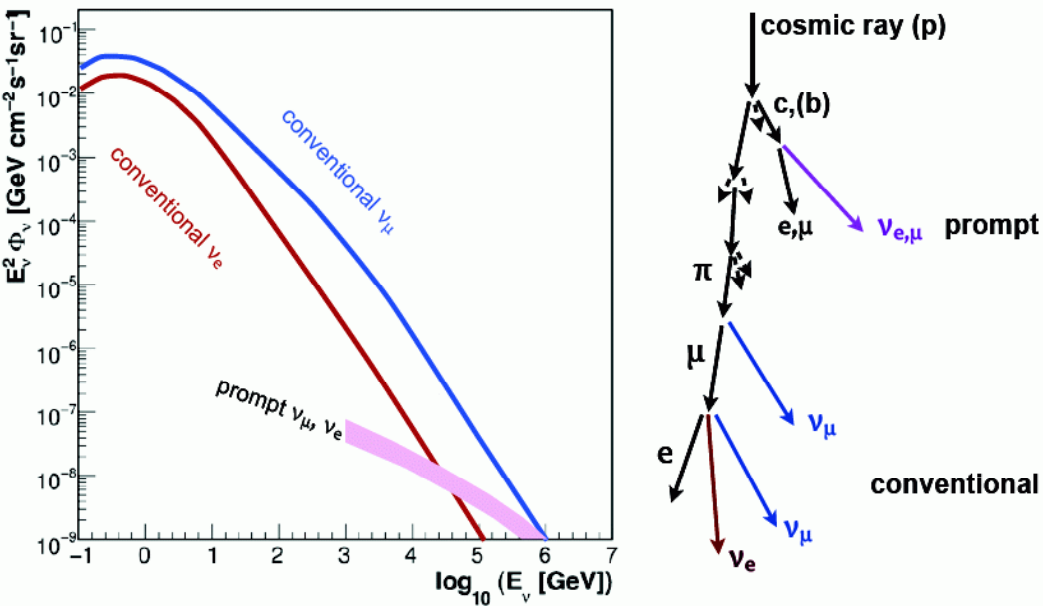
\includegraphics[width=0.5\linewidth]{neutrinos/kosmisch verval.png}
            \caption{Verval van kosmische straling in de atmosfeer}%
            \label{fig:neutrinos/kosmisch verval}
        \end{figure}

    \item Kern reactoren: Deze hebben energie in de orde van MeV's. In de nucleaire reactoren zijn er een hoop kernen aanwezig met een overmaat aan neutronen. Deze zetten een kettingreactie in gang waar de ene na de andere neutron rijke kern aan fissie productie doet. Dit is een $\beta^-$ verval $n \rightarrow p+e^{-}+\bar{\nu}_{e}$.
    \item Neutrino bundels: Deze worden gemaakt uit het verval van pion bundels $\pi \rightarrow \mu+\nu_{\mu} \rightarrow e+2 \nu_{\mu}+\nu_{e}$. De orde van de energie is in de GeV's.
\end{itemize}

\subsection{Zonne neutrino detectoren}%
\label{sub:zonne_neutrino_detectoren}

De allereerste detector om neutrinos te detecteren maakt gebruik van de het invers $\beta^-$ verval ($\bar{v}_{e}+p\rightarrow e^{+}+n$). In 1964 wordt dit geimplementeerd in het Homestake mine experiment. John Bacall is een theoretische astrofysicus die in detail uitrekende hoeveel neutrinos er uit de zon zouden moeten komen. Hij schat dat er enkele duizenden tot tienduizenden neutrinos per cm$^2$/s zouden moeten vrijkomen. Samen met Davis proberen ze dit nu te berekenen. Zoals gewoonlijk wordt dit voorstel afgewezen omdat het niet meetbaar zou zijn. Na bewijs dat het weldegelijk meetbaar is wordt het een 2de keer afgewezen omdat ze zeggen dat we toch weten uit berekeningen hoeveel neutrinos er uit de zon komen. Ze zijn hier toch mee verder gegaan met een groot vat aan droogkuisproduct. Hier zit chloor in dat de neutrinos kan opvangen.
\begin{equation}
    \begin{aligned}
        \label{eq:cl_neutrino_capture}
        \nu_{e}+^{37} \mathrm{Cl} \rightarrow^{37} \mathrm{Ar}+e^{-}
    \end{aligned}
\end{equation}
De threshold voor deze reactie is $E_\nu > 0.814$MeV. Het zou makkelijker zijn om het elektron van deze reactie te meten in plaats van het bubbeltje aan argon gas maar er zijn zo weinig evenementen dat het zo goed als onmogelijk is om deze waar te nemen.
\begin{equation}
    \begin{aligned}
        \label{eq:homestake_mine_exp}
        R(\mathrm{Cl}, S S M) &=8.1 \pm 1.3 S N U \\
        R(\mathrm{Cl}, \text { exp. }) &=2.56 \pm 0.16 \pm 0.16 S N U
    \end{aligned}
\end{equation}
$SNU$ is hier de solar neutrino unit. De foutenvlag van het standaard zonne model komt van de onzekerheden van de astrofysische modelen die we hebben van de zon. In het experiment zien we maar $30\%$ van de voorspelde neutrino flux.\\
De reacties hierop zijn voorspelbaar. Langs de ene kant wordt door theoretischi gezegd dat ze niet kunnen meten en de experimenticussen zeggen dat een slechte voorspelling is gemaakt. Als je zo een verschil ziet, probeer je het experiment opnieuw maar beter uit te voeren om zeker te zijn wat we hebben waargenomen.\\
Het is beter om dit experiment met gallium capture van neutrinos uit te voeren.
\begin{equation}
    \begin{aligned}
        \label{eq:ga_neutrino_capture}
        \nu_{e}+{ }^{71} \mathrm{Ga} \rightarrow{ }^{71} \mathrm{Ge}+e^{-}
    \end{aligned}
\end{equation}
Het voordeel bij deze reactie is dat de energie threshold kleiner is, $E_\nu = 0.233$MeV. Met deze threshold is het mogelijk om neutrinos uit de $pp$-cyclus waar te nemen. Het probleem bij dit experiment is dat gallium niet makkelijk te verkrijgen is en dus duur is. Dit onderzoek is gedaan in het GALLEX en SAGE experiment. SAGE staat voor soviet american gallium experiment. In 1992 is de Soviet unie gevallen en was het te gevaarlijk geworden om het SAGE experiment verder te zetten in het Caucasus gebergte. Het heeft geduurd tot eind  de jaren 90 om de zaken terug onder controle te krijgen. Hieruit kregen we terug dat er te weinig neutrinos werden waargenomen.\\
Het probleem bij dit soort experimenten was dat enkel het aantal waargenomen neutrinos werd geteld, niet hun richting. We waren dus niet zeker dat deze neutrinos van de zon kwamen. Het is dus nodig een experiment te ontwerpen die dit wel kan. Het Kamiokande experiment probeert de neutrinos waar te nemen aan de hand van elastische botsingen, $\nu_{x}+e^{-} \rightarrow \nu_{x}+e^{-}$. Hier is een gigantische hoeveelheid ultra zuiver water waar een elektron kan versneld worden aan de hand van de elastische botsing. Dit elektron zal in het water sneller dan het licht gaan en doet aan Cerenkov straling. Projecteer je deze straling op een detector dan krijg je Cerenkov ringen. Aan de hand van de grote van de ring kan een idee gekregen worden over de snelheid van het elektron. Belangrijker kan aan de hand van de orientatie van deze ring de richting van het elektron bepaald worden. Het nadeel hierbij is dat er hoge threshold energie nodig is. Zetten we het aantal evenementen nu uit in functie van de hoek naar de zon (figuur \ref{fig:neutrinos/kamiokande_results}) zien we duidelijk dat er een overschot is aan neutrinos die komen van de zon.

\begin{figure}[h]
    \centering
    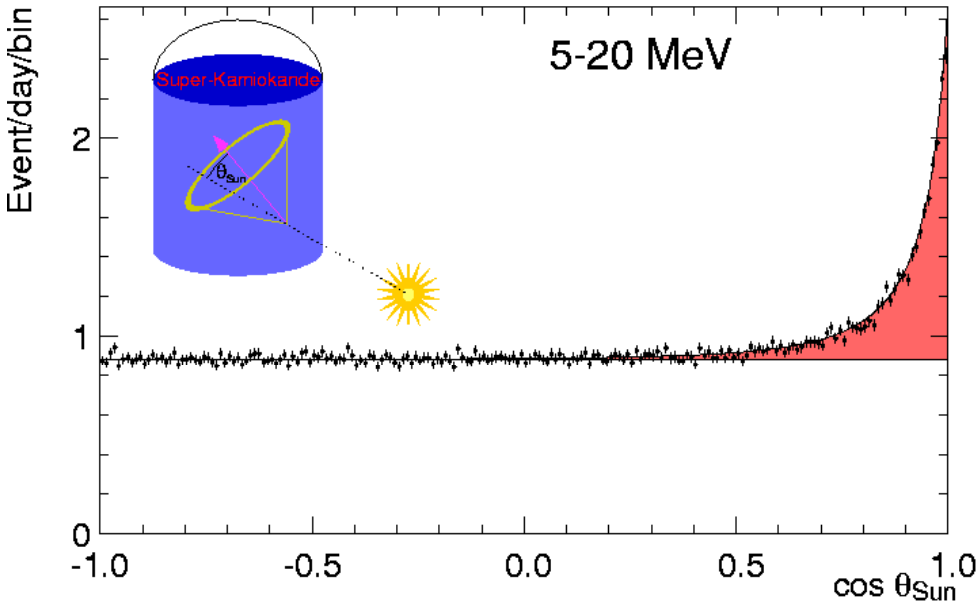
\includegraphics[width=0.5\linewidth]{neutrinos/kamiokande_results.png}
    \caption{Resultaten van het Kamiokande experiment}%
    \label{fig:neutrinos/kamiokande_results}
\end{figure}

\end{document}
